\documentclass{article}
\usepackage[utf8]{inputenc}
\usepackage{graphicx}

\title{Assignment 6: HMM}
\author{Avery Frankenberg}
\date{February 2019}

\begin{document}

\maketitle

\section{Hidden Markov Model Problem}
For this assignment our task was to create an HMM for a maze world. The paradigm is a 4x4 maze where every square in the maze has a colored tile on the floor. The robot does not know where it is or what direction it is moving, but it does know the layout of the maze (i.e. where the walls are and how big the maze is overall), and it receives sensor information about what color the tile it is currently on is. However, this sensor does not work perfectly; if the robot is on a red tile 88 percent of the time it returns red, 4 percent of the time it returns green, 4 percent of the time it returns blue, and 4 percent of the time it returns yellow. This property is symmetric, if the tile was blue then the sensor would return blue 88 percent of the time, etc. Our goal was to create a probability distribution of the possible states in the maze as the robot moves around and receives sensor stimuli.

To layout the problem, I modified some of the code from the maze world assignment for loading in mazes and processing them into a usable form. The file Maze.py takes a .maz file and processes it by creating a maze map, a color map, a color probability map, and obtaining the height and width of the maze. The maze map is created by calling the method create maze map. This turns the ASCII .maz file into an array representing where the walls and floor tiles are. The length of the array is the number of tiles there are in the maze. The color map is created by calling the method create color map. This method takes the list of colors read from the .maz file and turns them into the same length array as the maze map, except each value is the color of the tile at that specific location. The color probability map is a 2d array of the different color probabilities at a given location in the order ['r', 'g', 'b', 'y']. For example, if the color of the tile at (0, 0) is red then the list at that respective location would be [0.88, 0.04, 0.04, 0.04]. 

\section{Filtering}
To calculate this probability distribution I used a technique called filtering. This technique is implemented in the file HMM.py. From the Maze.py file the height, width, robot location, maze map, color map, and color map probabilities are all inherited. In the initialization, the start state is generated (which is an array of length 16 where every value is 1/16 or .0625), the update matrices are generated for each color, and the transition matrix is created. The update matrices are specific for the color that is perceived by the sensor. For each location in the maze, if the tile is actually that color then the value is 0.88 and if it is not that color then the value is .04. The update matrices are each 16x16 matrix where the diagonal contains the values that represent color perceived vs actual color, while every other value is 0. This allows for matrix multiplication in the filtering algorithm and pre-processing the matrices means that they won't have to be generated over and over as the algorithm runs.

The transition matrix is also a 16x16 matrix. It is created in the create transition matrix method. This method loops through every location and it calculates a transition vector by calling create transition vector. Within create transition vector, the method assumes the robot is at the input location and it attempts to move the robot N, S, E and W. If any of these new locations are outside of the board or a wall then a probability of 0.25 is not included in the transition vector for that new location (0.25 because there is equal likelihood that the robot moves N, S, E, or W). If the robot isn't able to move all 4 directions because of either a wall or the edge of the board, then a value is given to the input location as well. For example, say that a robot was at the north edge of the board and it could move every direction but north as moving north would put it off of the board. Therefore, all of the new locations resulting from moving S, E, and W would have the probability 0.25 in addition to the initial input location which would also have a value of 0.25.

In the filtering method, three other helper methods are used: move, sense, and normalize. The body of the method runs for a given number of iterations--specified in the method call. First, the robot itself moves; this is not actually "known" by the algorithm, but it is known to us so that we can check the efficacy of our predictive model. Next, the prediction step happens where the current state is updated by multiplying the transition matrix using the numpy matmul method. Third, the sense method is called which returns the sensed color of the square that the robot has just moved to. Then, the state matrix is multiplied by the update matrix for the specific color that was sensed. After this, the iteration is run again until the iter value is at max iterations. Once all of the iterations are complete, the matrix is normalized as we want all of the values to sum to 1. Because we are using matrix multiplication to do the predict and update steps, the normalization only needs to happen once at the end. To do this the normalize method is called--this method sums up all of the current values, calculates the factor that each value needs to be scaled by, and then updates each value in the state by multiplying by this scalar.

\section{Bonus}
\subsection{Viterbi Algorithm}
For an extension, I implemented the Viterbi algorithm for determining a most likely path for the robot to travel through the maze. To do this I created four additional methods, viterbi, get update matrix, backtrack, and process backtrack. The viterbi method does the actual most likely path search. In the method call it receives the sense list, i.e. the ordered list of colors sensed by the robot. Next it initializes the graph to be a list of an empty dictionary (that will soon contain the probability of a given state and the backpointer from that given state) and by initializing a variable to equal the start state of the maze. Next, it gets the first color in the sense list. With this color it determines the update matrix that should be used by passing the color to the get update matrix method and retrieving the matrix this method returns. It will either return update red, update green, update blue, or update yellow. It then adds all of the possible start locations to the dictionary. The probability or "p" value is the associated probability of seeing that start state multiplied by the probability of seeing the specific color sensed at that given state and the backpointer is None for all of the start states. 

After initializing this start state, the method then loops through the rest of the sense observations. For each sense, it first adds an empty dictionary element to the list. Then, it loops through all of the previous states and finds the largest transition value from that previous state to the current next state times the probability of seeing the correct color at that next state. After determining the max transition value and the best previous state associated with it, the element is added to the dictionary with its associated probability and with the backpointer indicating the best previous state. Once this loop has gone through all of the sensed colors, the viterbi algorithm is complete and the backtrack method is called. 
When the backtrack method is called, it is passed the complete viterbi dictionary and the total number of observations. It starts at the final observation and obtains the maximum probability at all of the final states. It adds the state that has this maximum probability to the path list, and then follows the backpointers from this state back to the start. When it reaches the start, the path is reversed and passed to the process path method. This method then turns the integer representations of the maze locations into actual (x, y) coordinates. After generating this processed list it is returned to the viterbi method and the list is printed out to the console for the user to see.  
In this way, the Viterbi Algorithm finds the most likely path through the graph given a sequence of observations. While this is a most likely path, if there are many tiles of there same color, or not many walls, there could be multiple of the most likely path through the maze. Therefore, this is just one of the optimal pathways and not the only one. 

\subsection{Testing of Filtering and Viterbi}
Here are two results form tests of two different small mazes. I only ran it for 3 iterations each so that I could easily capture the results in one screen shot and present them easily. There are a few important elements two note. First, the first maze is very simple. Even though the Viterbi algorithm does not return the exact path that the robot traveled, it returns an equally likely path (as there are no walls and the colors in all of the locations are the same). Also, in the filtering we can see how the normalization does not occur until the end (as only the final probabilities sum to 1). 

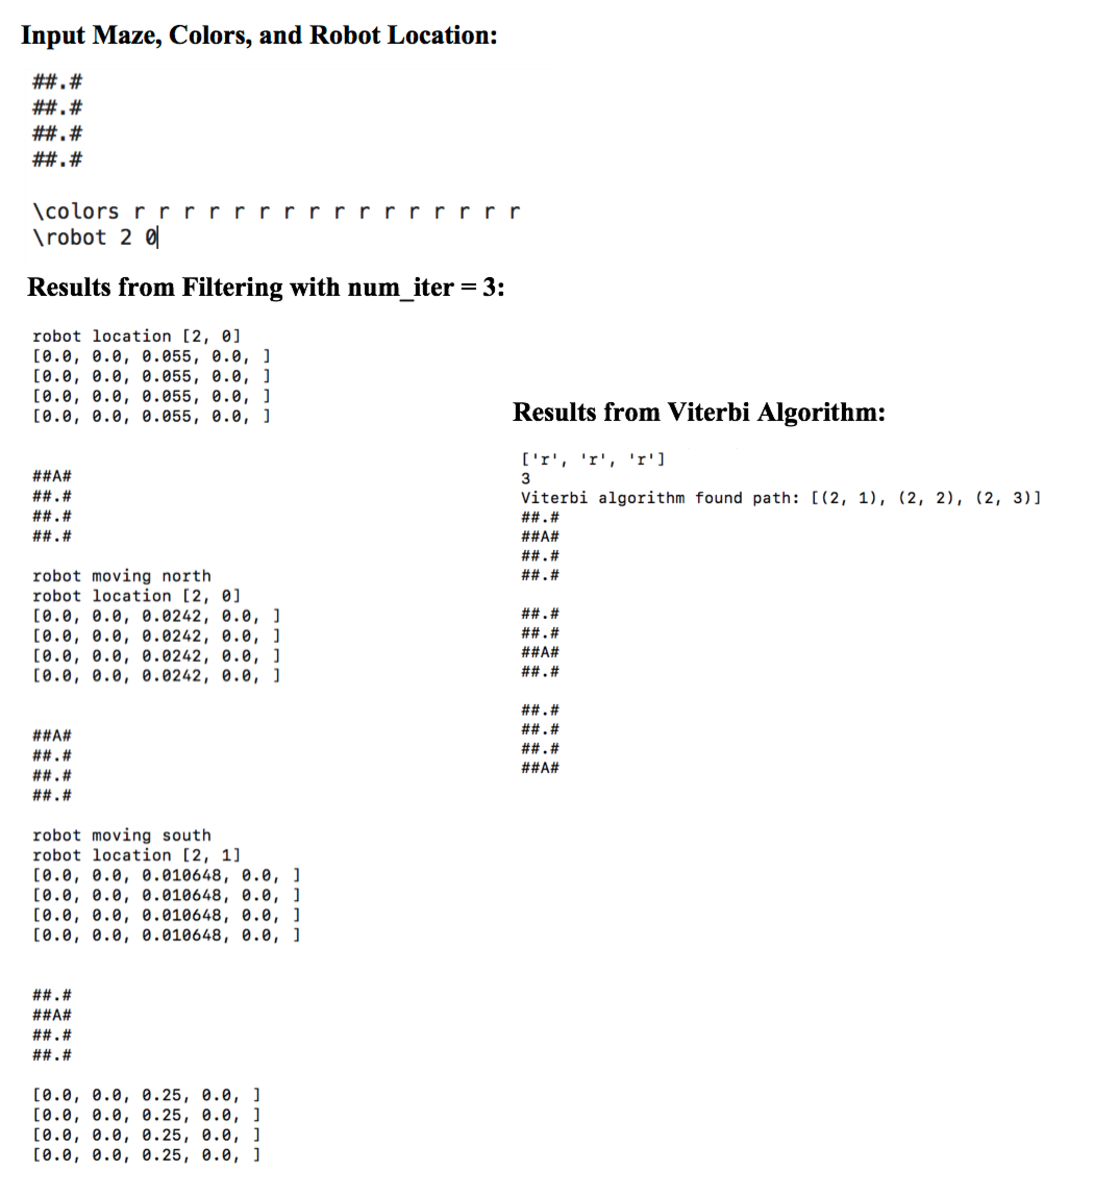
\includegraphics[width=\textwidth]{test_image_maze1.pdf}

In the second maze there are many more different colors and spaces the robot can move. We see that the robot can be in many more locations. However, 

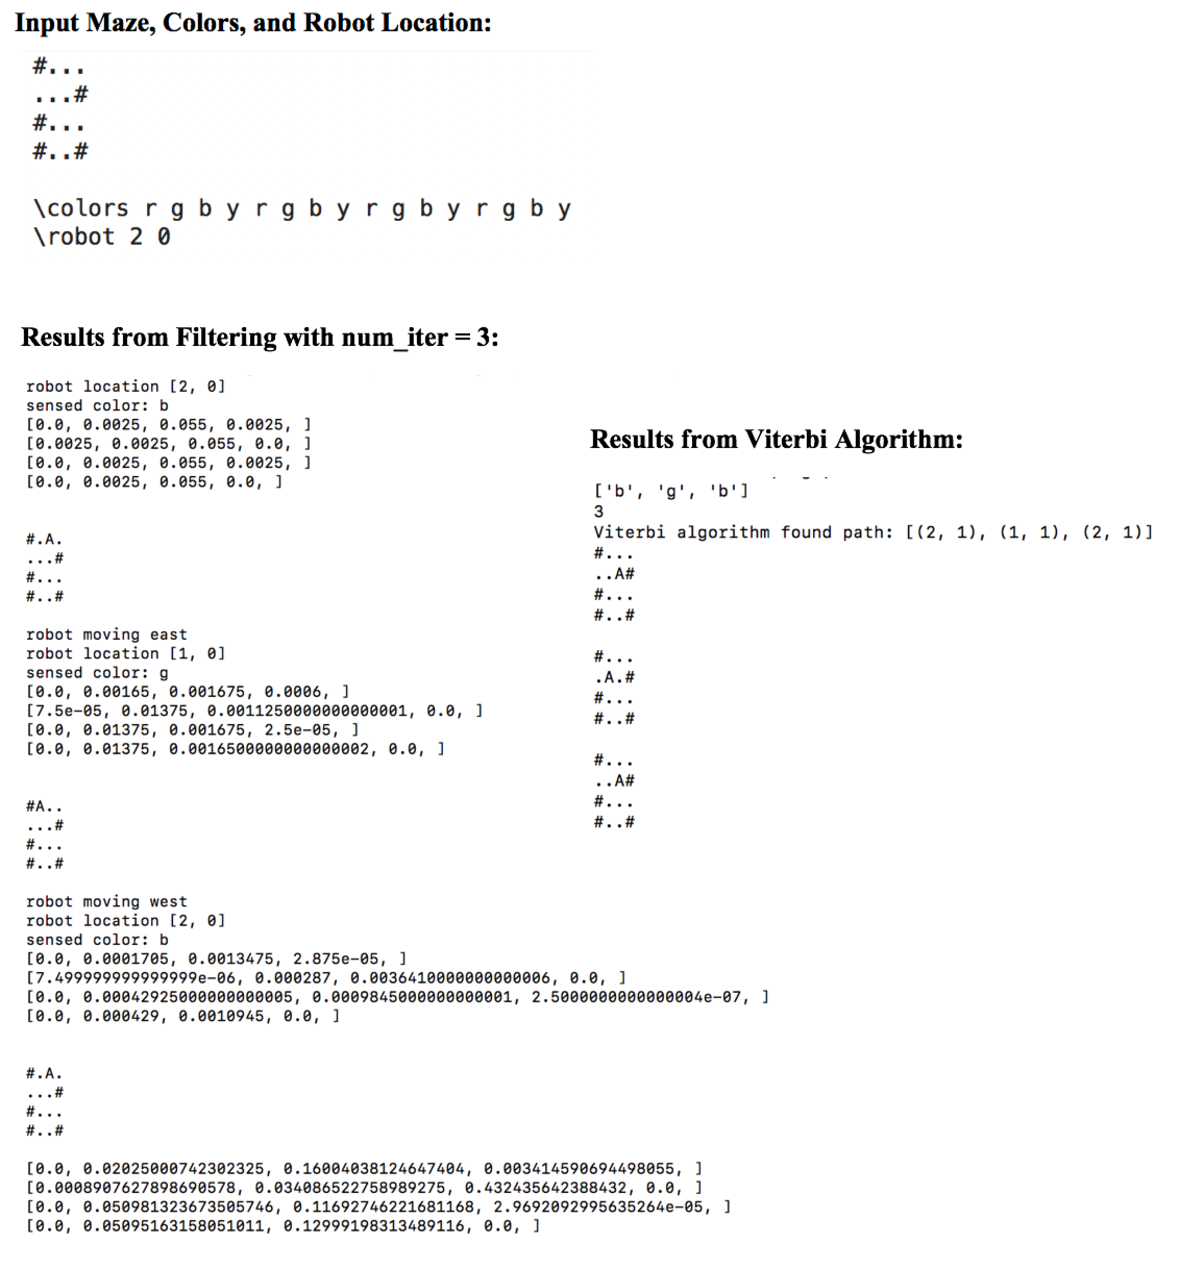
\includegraphics[width=\textwidth]{test_images_maze2.pdf}

\subsection{Forward Backward Smoothing}
For a second bonus, I implemented forward backward smoothing. Forward backward smoothing is the process of obtaining a better approximation of the state at a given time given observations both before and after the time desired. For example, we can approximate where the robot is at time t = 1 with the sensor and distribution information from time t = 0 and time t = 2. This gives us more information and therefore makes the approximation more accurate. To implement this I created five new methods: forward, backward, normalize, forward backward smoothing, and print smoothed state. The forward backward smoothing method is the method that is called in the test code and the one that runs the main algorithm. 

There are three parameters passed into the forward backward method, the evidence of the states, the prior (or initial state), and the index of the desired element. It also has three local variables, the forward messages stored in a list, the backward messages stored in a list, and the smoothed estimates stored in a list. The first element in the forward message is set to be the prior probabilities (the initial state of the maze). Then, a loop is run for each of the sensed colors provided, i.e. the number of evidence steps we have. In this loop the forward method is called, which calculates the probabilities of different states using the forward algorithm (which is basically the same as the backward algorithm). After the forward values are calculated, the backward loop is called. This loop starts at the end and goes until the beginning. The backward loop first sets the item at that index in the smoothed value list to be the matrix product between the forward vector at that index with the backward vector. Then the backward vector is updated by calling the backward method (which calculates a new probability distribution). This loop is completed for all of the evidence steps and then the smoothed vector is returned for the element, or time step, desired.

Below is the test code from the running of maze 2. Instead of running it with only 3 iterations, I ran it with 4. Below is the code from running the normal filtering algorithm, the Viterbi algorithm and the forward backward smoothing for obtaining the value at t = 1. In the results from the forward backward smoothing, we can see that the values are extremely high for being in the third column in the maze (element 2) at any height. This makes sense as the true sensed values were all blue and this column contains all blue squares. When comparing the values in this smoothed vector for time = 1 to the simply filtered values at time = 1, the probability of the robot being in this column (where the w value = 2), is much higher. This makes sense as the smoothed algorithm takes into account the fact that the robot senses blue the two steps after the desired time step as well as the time step before. 

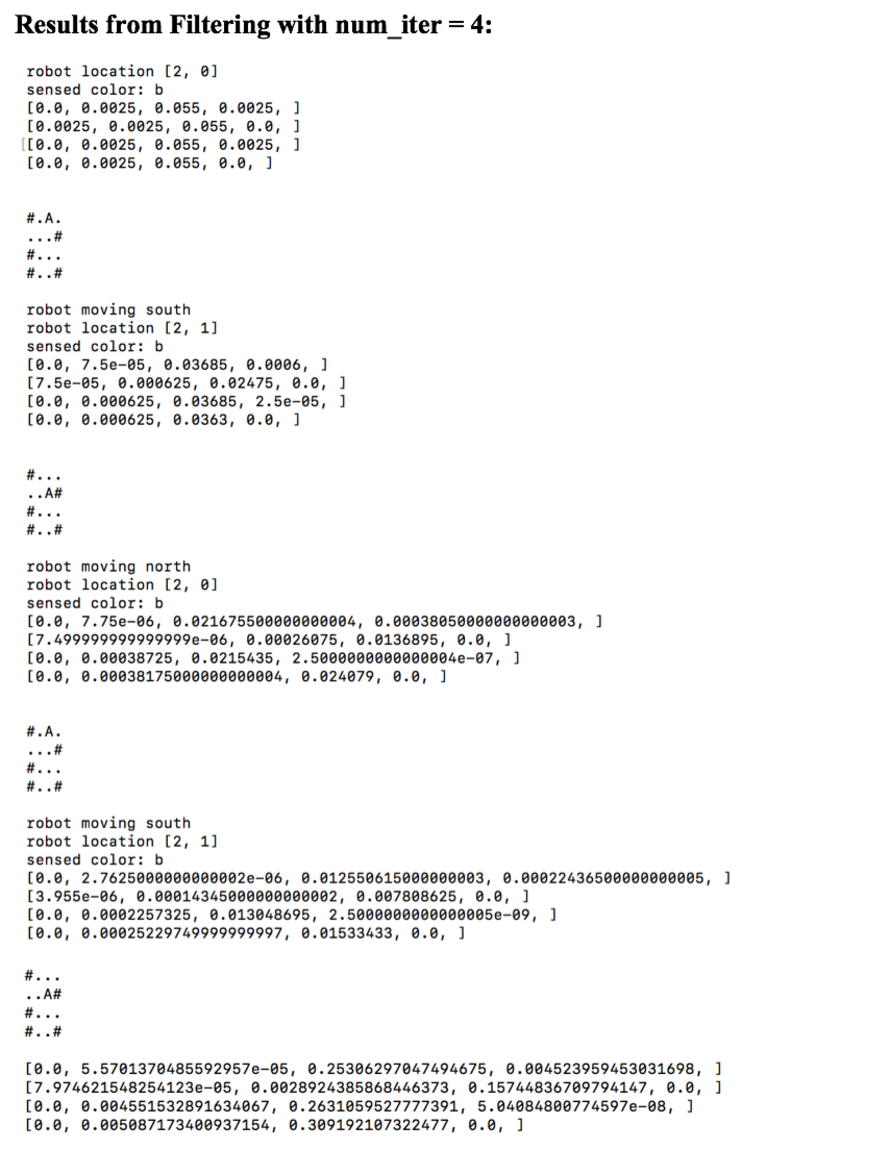
\includegraphics[width=\textwidth]{test_maze2_iter4.pdf}
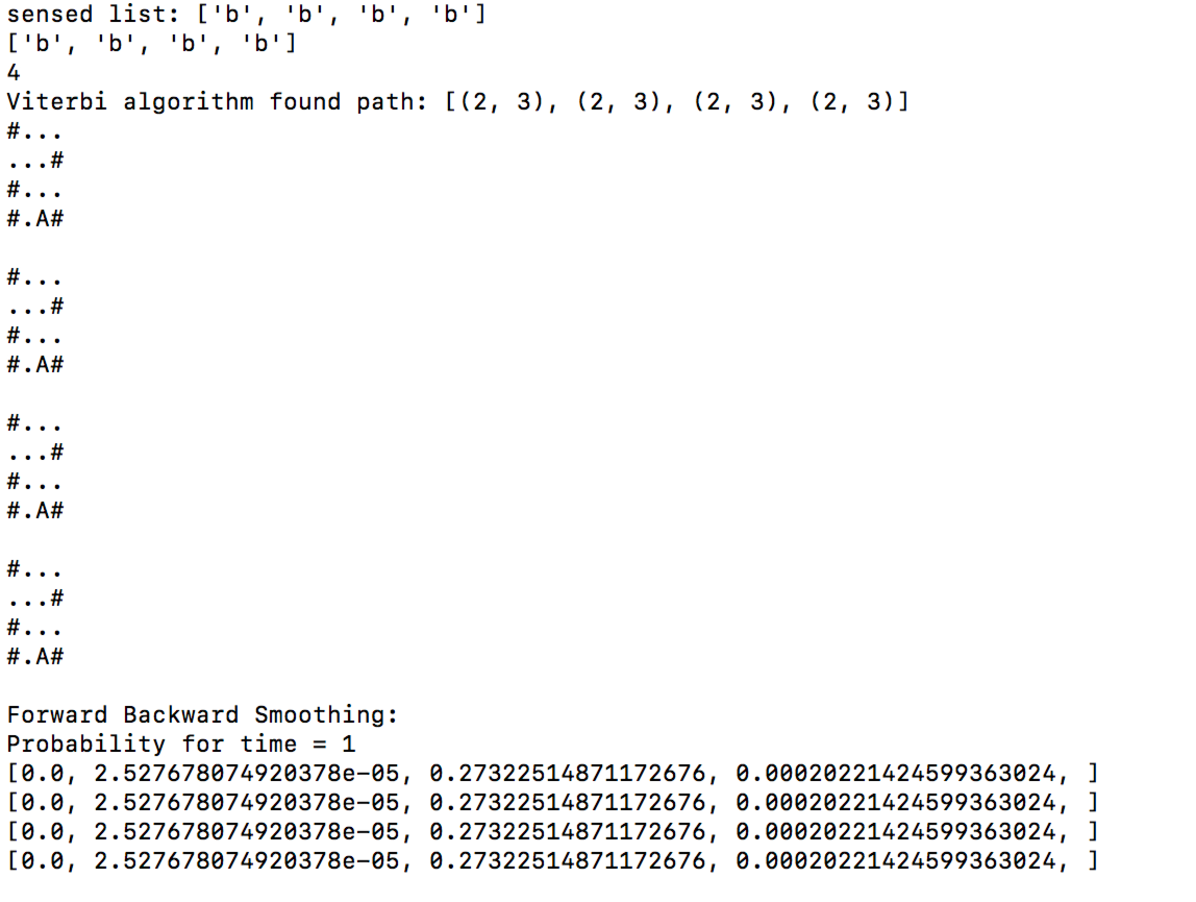
\includegraphics[width=\textwidth]{test_smoothing.pdf}

\end{document}
